
\centering
\begin{tikzpicture}[node distance=2.5cm]
	%tikzstyle{every node}=[font=\small]
	
	\rootnode;
	
	\withchildren{root}{n8}{$f(a) \neq f(b)$}{n7}{$f(a) = f(b)$};
	
	\withchildren{n7}{n5}{$b \neq f(b), f(a) = f(b)$}{n6}{$b = f(b)$};
	
	\withchildren{n5}{n3}{$a \neq b, b \neq f(b), f(a) = f(b)$}{n4}{$a = b$};
	
	\proofnode[above left of=n3]{n2}{$f(a) \neq a,a \neq b, b \neq f(b), f(a) = f(b)$};
	\proofnode[above right of=n3, xshift=1cm]{n1}{$f(a) = a$};
	\drawchildren{n3}{n1}{n2};
\end{tikzpicture}

